



\begin{frame}{OpenCL Library Ecosystem}

 \begin{minipage}{0.19\textwidth}
Abacus\\
ACML\\
Accelerate\\
amgCL\\
Aparapi\\
AQUAgpusph\\
ArrayFire\\
ASL\\
Barracuda\\
Bolt\\
Boost.Compute\\
Bullet Physics\\
C++ AMP\\
CALDGEMM\\
CF4OCL\\
clBLAS\\
clFFT\\
 \end{minipage}
 \begin{minipage}{0.19\textwidth}
CLFORTRAN\\
clMAGMA\\
clpp\\
clSpMV\\
CLTune\\
Clyther\\
Concord\\
COPRTHR\\
Data Layout\\
DelphiOpenCL\\
ForOpenCL\\
fortranCL\\
FSCL.Compiler\\
GMAC\\
Go-OpenCL\\
GPULib\\
gpumatrix\\
 \end{minipage}
  \begin{minipage}{0.2\textwidth}
GPUVerify\\
Halide\\
Harlan\\
Haskell\\
HOpenCL\\
JOCL\\
libCL\\
Libra SDK\\
Lua\\
M3\\
MUMPS\\
Octave\\
OpenFortranP.\\
OpenCL.jl\\
OpenCL.NET\\
OpenCLIPP\\
OpenCLLink\\
 \end{minipage}
  \begin{minipage}{0.20\textwidth}
OpenClooVision\\
OpenCV-CL\\
OpenHMPP\\
Paralution\\
Pardiso\\
Pencil\\
PETSc\\
PyOpenCL\\
RaijinCL\\
Rivertrail\\
RNG\\
ROpenCL\\
RoseACC-OpenCL\\
Rose Compiler\\
Rust-OpenCL\\
ScalaCL\\
 \end{minipage}
  \begin{minipage}{0.19\textwidth}
SkelCL\\
SnuCL\\
SpeedIT 2.4\\
streamscan\\
SuperLU\\
s-u/OpenCL\\
TM-Task\\
Trilinos\\
VexCL\\
ViennaCL\\
ViNN\\
VirtualCL\\
VOBLA\\
VOCL\\
VSI/Pro\\
WAMS\\
 \\
 \end{minipage}
 
 \begin{center}
  83 libraries listed on iwocl.org
 \end{center}
 
\end{frame}

%%%%% Remove dead, duplicates, and transitives

\begin{frame}{OpenCL Library Ecosystem}

 \begin{minipage}{0.19\textwidth}
Abacus\\
ACML\\
Accelerate\\
amgCL\\
Aparapi\\
AQUAgpusph\\
ArrayFire\\
ASL\\
Barracuda\\
Bolt\\
Boost.Compute\\
Bullet Physics\\
C++ AMP\\
CALDGEMM\\
 \end{minipage}
 \begin{minipage}{0.19\textwidth}
CF4OCL\\
clBLAS\\
clFFT\\
CLFORTRAN\\
clMAGMA\\
clpp\\
clSpMV\\
CLTune\\
Clyther\\
COPRTHR\\
Data Layout\\
DelphiOpenCL\\
ForOpenCL\\
fortranCL\\
 \end{minipage}
  \begin{minipage}{0.2\textwidth}
FSCL.Compiler\\
GMAC\\
Go-OpenCL\\
GPULib\\
gpumatrix\\
Halide\\
Harlan\\
Haskell\\
HOpenCL\\
JOCL\\
libCL\\
Libra SDK\\
Lua\\
M3\\
 \end{minipage}
  \begin{minipage}{0.20\textwidth}
OpenCL.jl\\
OpenCL.NET\\
OpenCLIPP\\
OpenCLLink\\
OpenClooVision\\
OpenCV-CL\\
OpenHMPP\\
Paralution\\
PyOpenCL\\
RaijinCL\\
Rivertrail\\
RNG\\
ROpenCL\\
Rose-OpenCL\\
 \end{minipage}
  \begin{minipage}{0.19\textwidth}
Rust-OpenCL\\
ScalaCL\\
SkelCL\\
SnuCL\\
SpeedIT 2.4\\
streamscan\\
s-u/OpenCL\\
TM-Task\\
VexCL\\
ViennaCL\\
ViNN\\
VirtualCL\\
VOBLA\\
 \\
 \end{minipage}
 
 \begin{center}
  69 libraries from iwocl.org still accessible, no transitives
 \end{center}
 
\end{frame}

%%%%% Remove inactive

\begin{frame}{OpenCL Library Ecosystem}

 \begin{minipage}{0.19\textwidth}
Abacus\\
ACML\\
Accelerate\\
amgCL\\
Aparapi\\
AQUAgpusph\\
ArrayFire\\
ASL\\
Bolt\\
Boost.Compute\\
Bullet Physics\\
 \end{minipage}
 \begin{minipage}{0.19\textwidth}
C++ AMP\\
CALDGEMM\\
CF4OCL\\
clBLAS\\
clFFT\\
CLFORTRAN\\
CLTune\\
COPRTHR\\
Data Layout\\
FSCL.Compiler\\
GMAC\\
 \end{minipage}
  \begin{minipage}{0.2\textwidth}
GPULib\\
Halide\\
Harlan\\
HOpenCL\\
JOCL\\
libCL\\
Libra SDK\\
Lua\\
M3\\
OpenCL.jl\\
OpenCLIPP\\
 \end{minipage}
  \begin{minipage}{0.20\textwidth}
OpenCLLink\\
OpenCV-CL\\
Paralution\\
PyOpenCL\\
RaijinCL\\
Rivertrail\\
RNG\\
ROpenCL\\
Rose-OpenCL\\
Rust-OpenCL\\
ScalaCL\\
 \end{minipage}
  \begin{minipage}{0.19\textwidth}
SkelCL\\
SnuCL\\
SpeedIT 2.4\\
TM-Task\\
VexCL\\
ViennaCL\\
ViNN\\
VirtualCL\\
VOBLA\\
 \\
 \\
 \end{minipage}
 
 \begin{center}
  53 active libraries (based on list at iwocl.org)
 \end{center}
 
\end{frame}



%%%%% Split off bindings

\begin{frame}{OpenCL Library Ecosystem}

 \begin{minipage}{0.49\textwidth}
 \begin{block}{Bindings (18)}\end{block}
 \begin{minipage}{0.49\textwidth}
Aparapi\\
CF4OCL\\
CLFORTRAN\\
FSCL.Compiler\\
Halide\\
Harlan\\
HOpenCL\\
JOCL\\
Lua\\
OpenCL.jl\\
OpenCLIPP\\
OpenCLLink\\
PyOpenCL\\
Rivertrail\\
ROpenCL\\
Rose-OpenCL\\
Rust-OpenCL\\
ScalaCL\\
 \end{minipage}
  
 \end{minipage}
 \begin{minipage}{0.49\textwidth}
 \begin{block}{Algorithms (35)}\end{block}
 \begin{minipage}{0.49\textwidth}
Abacus\\
ACML\\
Accelerate\\
amgCL\\
AQUAgpusph\\
ArrayFire\\
ASL\\
Bolt\\
Boost.Compute\\
Bullet Physics\\
C++ AMP\\
CALDGEMM\\
clBLAS\\
clFFT\\
CLTune\\
COPRTHR\\
Data Layout\\
GMAC\\
 \end{minipage}
  \begin{minipage}{0.49\textwidth}
GPULib\\
libCL\\
Libra SDK\\
M3\\
OpenCV-CL\\
Paralution\\
RaijinCL\\
RNG\\
SkelCL\\
SnuCL\\
SpeedIT 2.4\\
TM-Task\\
VexCL\\
ViennaCL\\
ViNN\\
VirtualCL\\
VOBLA\\
 \\
 \end{minipage}
    
 \end{minipage}

 \begin{center}
 \vspace*{-.5cm} \scriptsize (based on list at iwocl.org, filtering applied)
 \end{center}

\end{frame}


%%%%%%%%% Split off Linear Algebra

%%%%% Split off bindings

\begin{frame}{OpenCL Library Ecosystem}

 \begin{minipage}{0.24\textwidth}
 \begin{block}{Bindings (18)}
Aparapi\\
CF4OCL\\
CLFORTRAN\\
FSCL.Compiler\\
Halide\\
Harlan\\
HOpenCL\\
JOCL\\
Lua\\
OpenCL.jl\\
OpenCLIPP\\
OpenCLLink\\
PyOpenCL\\
Rivertrail\\
ROpenCL\\
Rose-OpenCL\\
Rust-OpenCL\\
ScalaCL\\
\end{block}  
 \end{minipage}
 \begin{minipage}{0.24\textwidth}
 \begin{block}{Math (14)}
Abacus\\
ACML\\
amgCL\\
ArrayFire\\
CALDGEMM\\
clBLAS\\
GPULib\\
Paralution\\
RaijinCL\\
SkelCL\\
SpeedIT 2.4\\
VexCL\\
ViennaCL\\
VOBLA\\  
 \\
 \\
 \\
 \\
 \end{block}
  \end{minipage}
 \begin{minipage}{0.24\textwidth}
 \begin{block}{Primitives (7)}
Bolt\\
Boost.Compute\\
clFFT\\
CLTune\\
libCL\\
M3\\
RNG\\
 \\
 \\
 \\
 \\
 \\
 \\
 \\
 \\
 \\
 \\
 \\
 \end{block}
  \end{minipage}
 \begin{minipage}{0.24\textwidth}
 \begin{block}{Other (14)}
Accelerate\\
AQUAgpusph\\
ASL\\
Bullet Physics\\
C++ AMP\\
COPRTHR\\
Data Layout\\
GMAC\\
Libra SDK\\
OpenCV-CL\\
SnuCL\\
TM-Task\\
ViNN\\
VirtualCL\\
 \\
 \\
 \\
 \\
 \end{block}
 \end{minipage}
 
 \begin{center}
 \vspace*{-.5cm} \scriptsize (based on list at iwocl.org, filtering applied)
 \end{center}

\end{frame}



\begin{frame}{OpenCL vs. CUDA for Libraries}

 \begin{block}{OpenCL}
   \begin{itemize}
    \item Header and shared library
    \item Non-intrusive to build system
    \item jit-compilation
   \end{itemize}
 \end{block}

 %\pause
 \begin{block}{CUDA}
   \begin{itemize}
    \item Custom compiler wrapper (NVCC)
    \item NVCC dictates your host compiler
    \item Single source
    \item Kernel binaries embedded in executable
   \end{itemize}
 \end{block}

 %\pause
 \begin{block}{How about SyCL?}
   \begin{itemize}
    \item Bring single-source approach to OpenCL
    \item jit-compilation
   \end{itemize}
 \end{block}

\end{frame}


\begin{frame}{Outline}
\begin{center}
 {\Large How can we make OpenCL more library-friendly?}
\end{center}
\end{frame}


\begin{frame}{Outline}

 \begin{block}{Just-In-Time Kernel Compilation}
   \begin{itemize}
    \item Library may provide hundreds of kernels
    \item Just-in-time compilation entails certain overhead
   \end{itemize}
 \end{block}

 %\pause
 \begin{block}{Kernel Interaction}
   \begin{itemize}
    \item Host-function not callable from OpenCL kernel on host
    \item Hindrance to software composability
   \end{itemize}
 \end{block}

 %\pause
  \begin{block}{OpenCL Heterogeneity}
   \begin{itemize}
    \item OpenCL 2.2 was released this week
    \item Many SDKs still at OpenCL 1.2 or earlier
   \end{itemize}
 \end{block}
\end{frame}


%%% Say what is not included in the talk
% - performance portability
% - compiler bugs

\begin{frame}{Not In This Talk}

 \begin{block}{Performance Portability}
   \begin{itemize}
    \item Not specific to libraries
    \item Several strategies proposed in the past
   \end{itemize}
 \end{block}
 \vspace*{.5cm}
 
 %\pause
 \begin{center}
  \textit{``There is no secret to performance portability;\\
          it's just hard.``} --- Neil Trevett, IWOCL 2016
 \end{center}

 
 %\pause
 \vspace*{.5cm}
  \begin{block}{ViennaCL Approach}
   \begin{itemize}
    \item Extensive kernel parameterization
    \item Built-in device database
    \item Match device type, vendor, architecture, device name
   \end{itemize}
 \end{block}
\end{frame}


%%% Kernel compilation



\begin{frame}[fragile]{Just-In-Time Kernel Compilation}

 \begin{block}{Kernel Compilation}
   \begin{itemize}
    \item Library may provide hundreds of kernels
    \item Just-in-time compilation entails certain overhead
   \end{itemize}
 \end{block}

 \begin{block}{Little Experiment}
  \begin{itemize}
   \item Compile 64 trivial kernels of the form
   \begin{lstlisting}
__kernel void kernel_1_2(__global float *x){ x[1] = 2; }
   \end{lstlisting}
   \item Organize in 1 to 64 programs for 64 to 1 kernels each
  \end{itemize}
 \end{block}
 
\end{frame}




\begin{frame}{Just-In-Time Kernel Compilation}
\begin{center}
 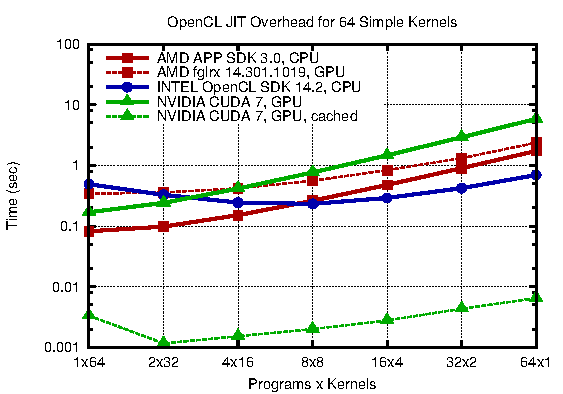
\includegraphics[width=0.95\textwidth]{figures/jit-overhead-5}
\end{center}
\end{frame}


\begin{frame}[fragile]{Just-In-Time Kernel Compilation}

 \begin{block}{OpenCL Program Cache}
   \begin{itemize}
    \item Compiled binaries stored in filesystem
    \item Implement in $\mathcal{O}(10)$ OpenCL SDKs?
    \item Implement in $\mathcal{O}(100)$ OpenCL-based libraries?
   \end{itemize}
 \end{block}

 \begin{block}{Proposed Solution}
   \begin{itemize}
    \item Make kernel caching a required (optional) feature for OpenCL SDKs
   \end{itemize}
 \end{block}

\end{frame}



\begin{frame}[fragile]{Just-In-Time Kernel Compilation}

 \begin{block}{SyCL to the Rescue?}
   \begin{itemize}
    \item SyCL compiler cannot generate binaries for all possible targets
    \item jit-overhead still an issue (unlike CUDA)
   \end{itemize}
 \end{block}

 \begin{block}{SPIR-V to the Rescue?}
   \begin{itemize}
    \item May reduce jit-compilation overhead substantially
    \item Broad availability required
   \end{itemize}
 \end{block}

\end{frame}



%%% Extensibility (callbacks)



\begin{frame}[fragile]{Kernel Interaction}

 \begin{block}{Composability}
   \begin{itemize}
    \item Mix and match functionality in different libraries
    \item Basic entity: function calls
   \end{itemize}
 \end{block}
 
% Motivating example: sort
 %\pause
 \begin{block}{Example: Sorting}
  \begin{lstlisting}
 void sort_criterion(...) { /* tricky criterion */ }
 std::sort(x.begin(), x.end(), sort_criterion);
  \end{lstlisting}
 \end{block}

  %\pause
  \begin{block}{OpenCL on CPU}
   \begin{itemize}
    \item Plethora of libraries for host available
    \item Easy to call OpenCL libraries from host
    \item (Almost) Impossible to call host libraries from OpenCL kernel
   \end{itemize}
 \end{block}
 
\end{frame}


% Show figure: Diode effect of OpenCL

\begin{frame}[fragile]{Kernel Interaction}

\begin{center}
  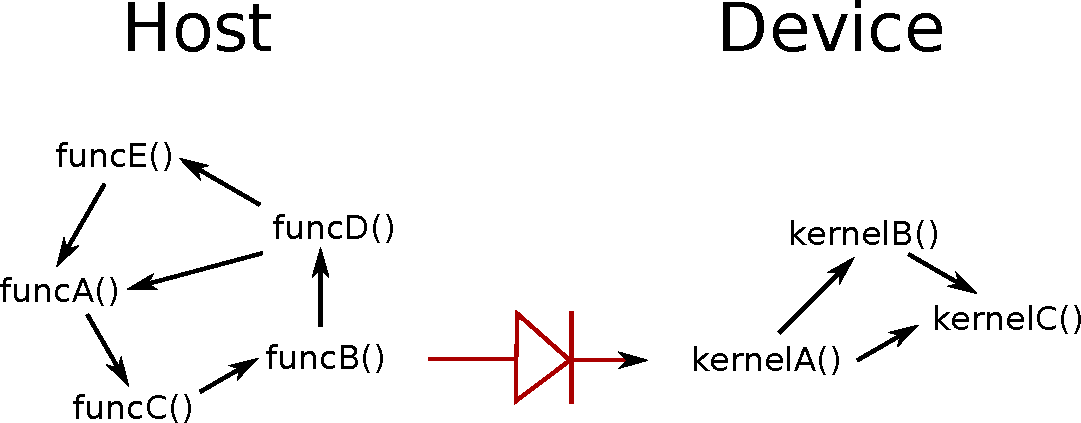
\includegraphics[width=0.9\textwidth]{figures/diode}
\end{center}

 %\pause
 \begin{block}{Proposed Improvement}
   \begin{itemize}
    \item Allow calling host functions for OpenCL kernels on CPU
   \end{itemize}
 \end{block}
  
\end{frame}





%%% Heterogeneous OpenCL versions 
%% 9. OpenCL

\begin{frame}{History of OpenCL}

\begin{minipage}{0.7\textwidth}
\begin{block}{Prior to 2008}
  \begin{itemize}
   \item OpenCL developed by Apple Inc.
  \end{itemize}
\end{block}

\begin{block}{2008}
  \begin{itemize}
   \item OpenCL working group formed at Khronos Group
   \item OpenCL specification 1.0 released
  \end{itemize}
\end{block}

\begin{block}{2010}
  \begin{itemize}
   \item OpenCL 1.1 (multi-device, subbuffer manipulation)
  \end{itemize}
\end{block}

\begin{block}{2011}
  \begin{itemize}
   \item OpenCL 1.2 (device partitioning)
  \end{itemize}
\end{block}

\begin{block}{2013}
  \begin{itemize}
   \item OpenCL 2.0 (shared virtual memory, SPIR, etc.)
  \end{itemize}
\end{block}

\end{minipage} \hfill
\begin{minipage}{0.25\textwidth}
 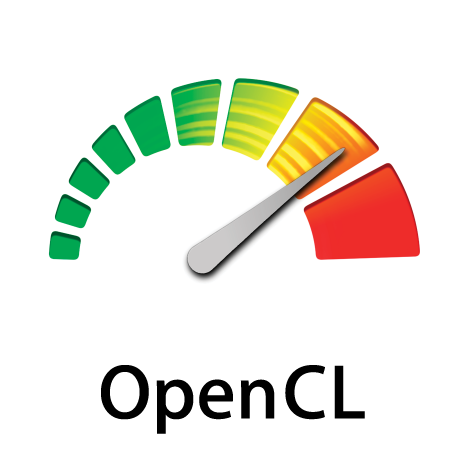
\includegraphics[width=0.99\textwidth]{figures/opencl.jpg}
 
 \vspace*{5cm}
\end{minipage}


\end{frame}


\begin{frame}{OpenCL}

\begin{block}{Similar to CUDA}
  \begin{itemize}
   \item Kernel language is a subset of C
   \item Explicit memory management, host-device transfers
   \item Memory model: local, shared, global
  \end{itemize}
\end{block}


\begin{block}{Different from CUDA}
  \begin{itemize}
   \item Support by many vendors
   \item No compiler-wrapper, only a shared library
   \item Kernel compilation usually at runtime
  \end{itemize}
\end{block}

\end{frame}

%%%%%%%%%%%%%%

% \begin{frame}{OpenCL Platform Model}
%  \begin{center}
%    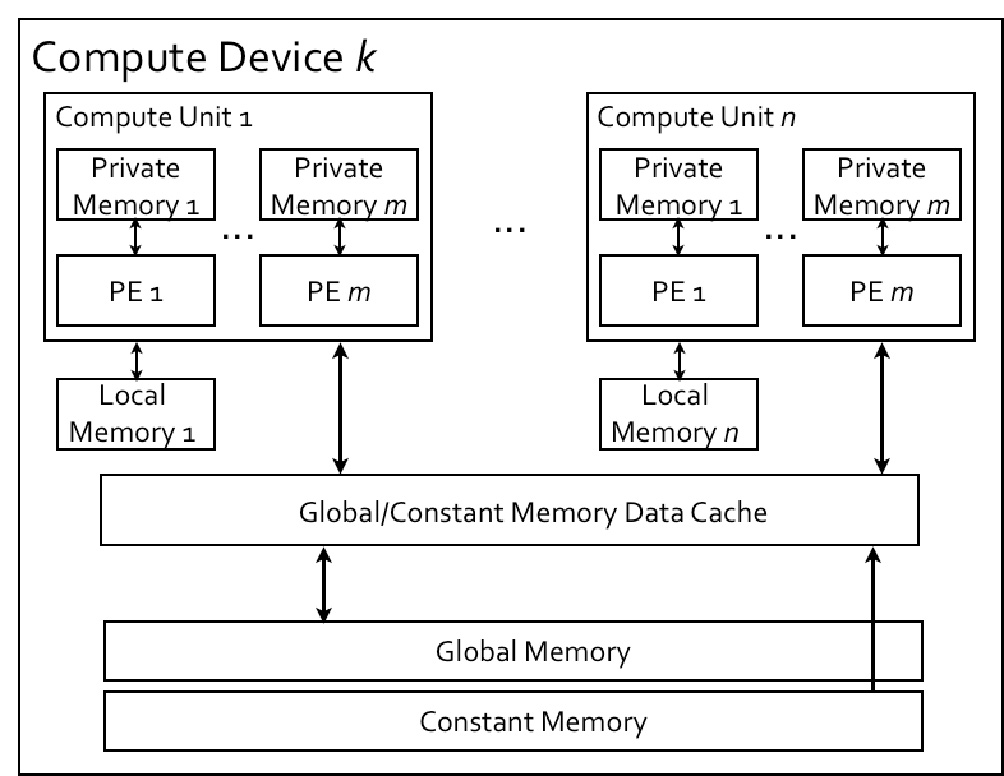
\includegraphics[width=0.80\textwidth]{figures/opencl-device}
%  \end{center}
% \end{frame}

%%%%%%%%%%%%%%%%%%%% Platform Model %%%%%%%%%%%%%%%%%%%%%%

% \begin{frame}{OpenCL Platform Model}
%  \begin{center}
%    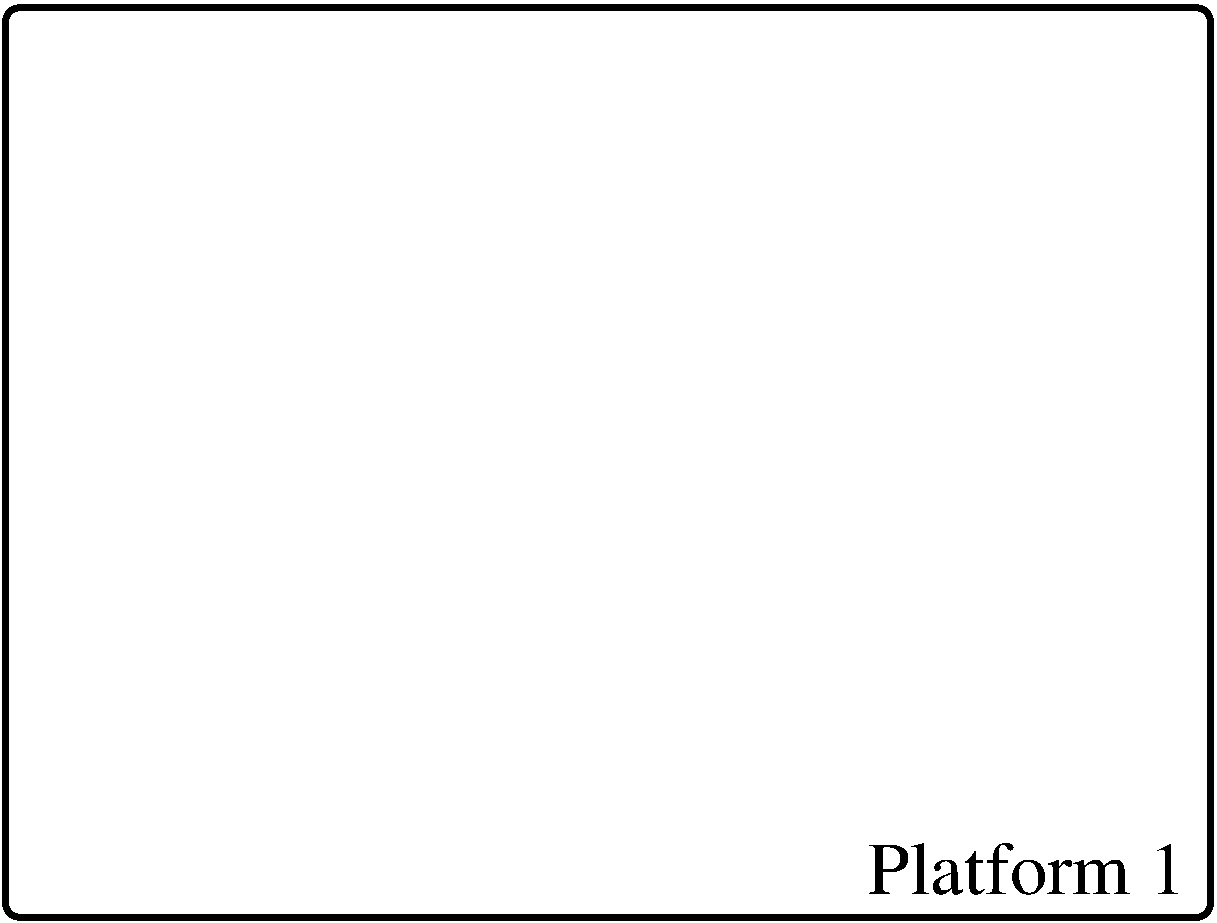
\includegraphics[width=0.80\textwidth]{figures/opencl-2.pdf}
%  \end{center}
% \end{frame}
% 
% \begin{frame}{OpenCL Platform Model}
%  \begin{center}
%    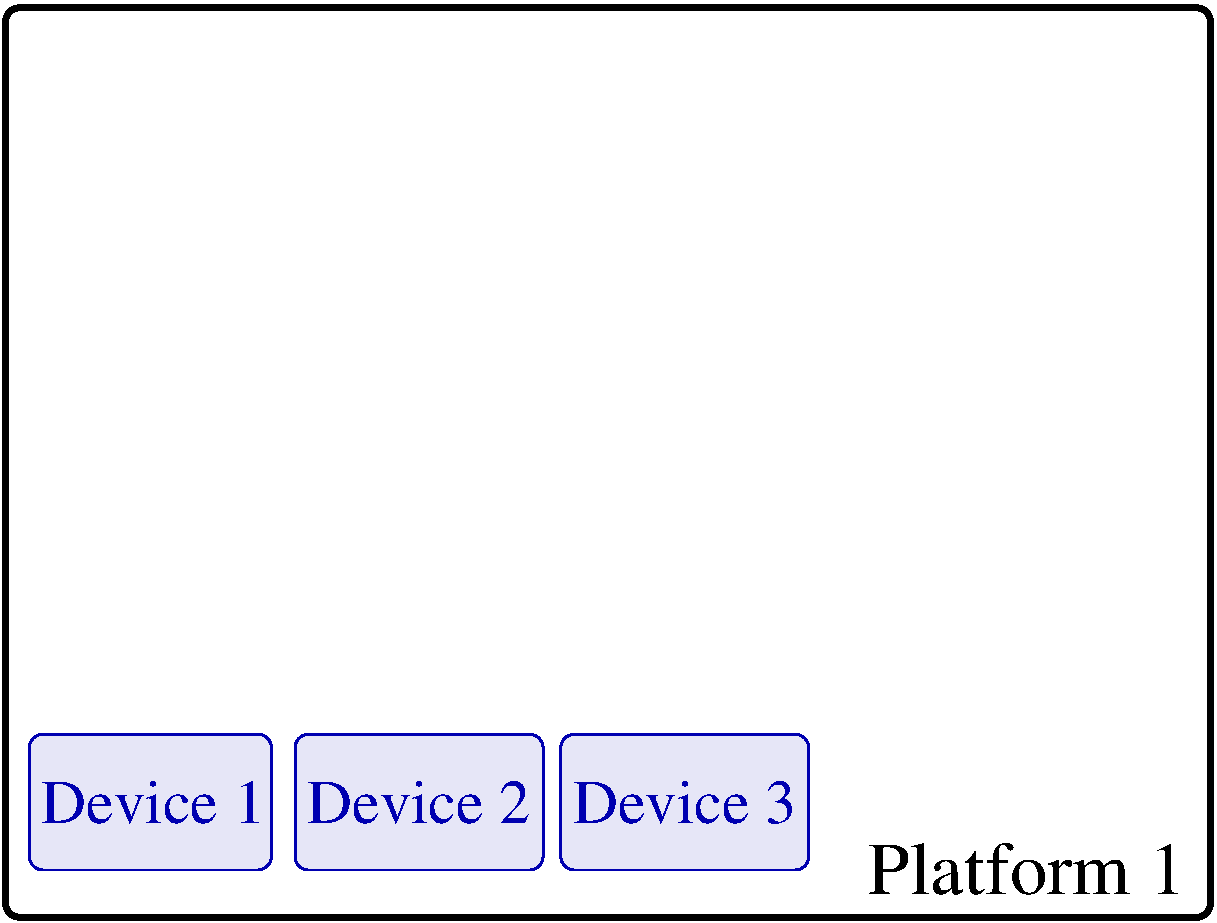
\includegraphics[width=0.80\textwidth]{figures/opencl-3.pdf}
%  \end{center}
% \end{frame}
% 
% \begin{frame}{OpenCL Platform Model}
%  \begin{center}
%    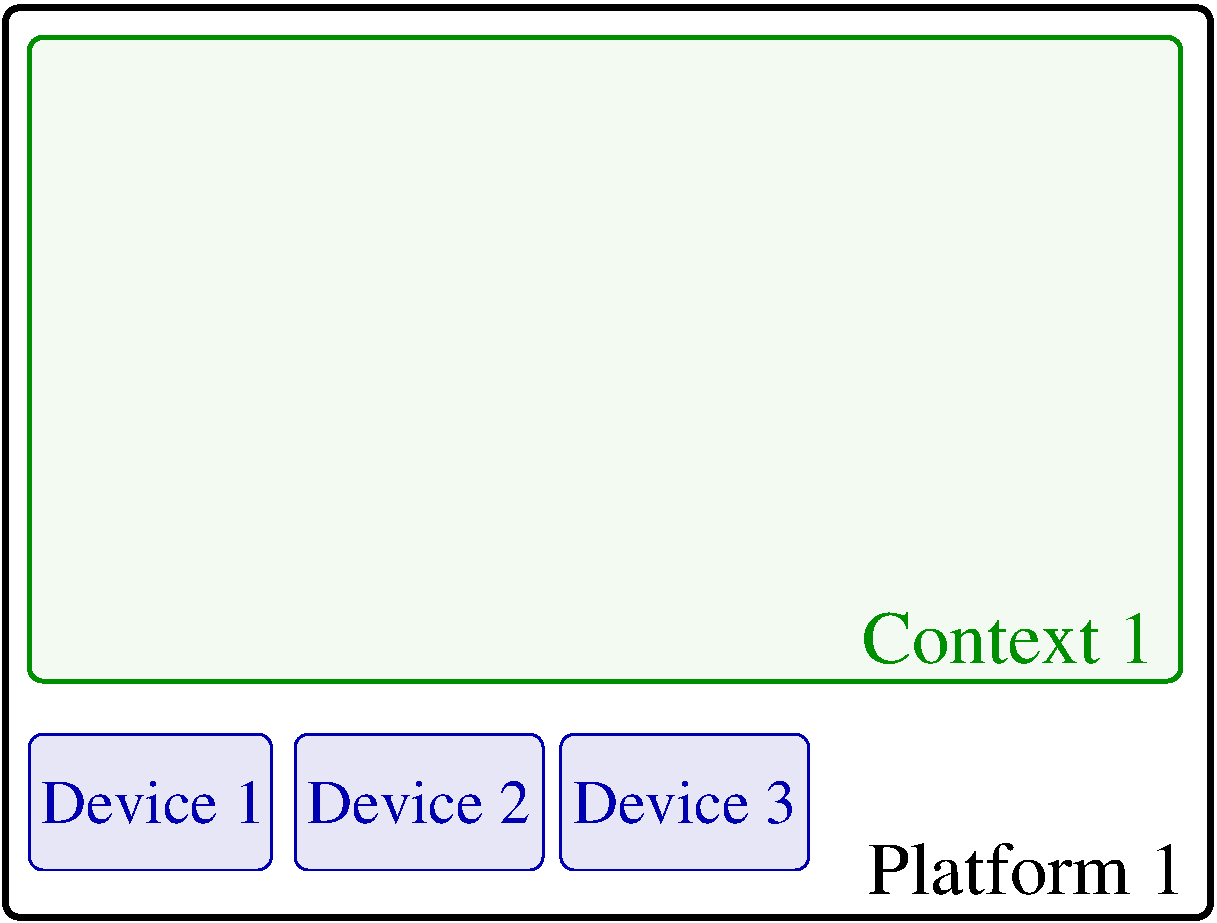
\includegraphics[width=0.80\textwidth]{figures/opencl-4.pdf}
%  \end{center}
% \end{frame}
% 
% \begin{frame}{OpenCL Platform Model}
%  \begin{center}
%    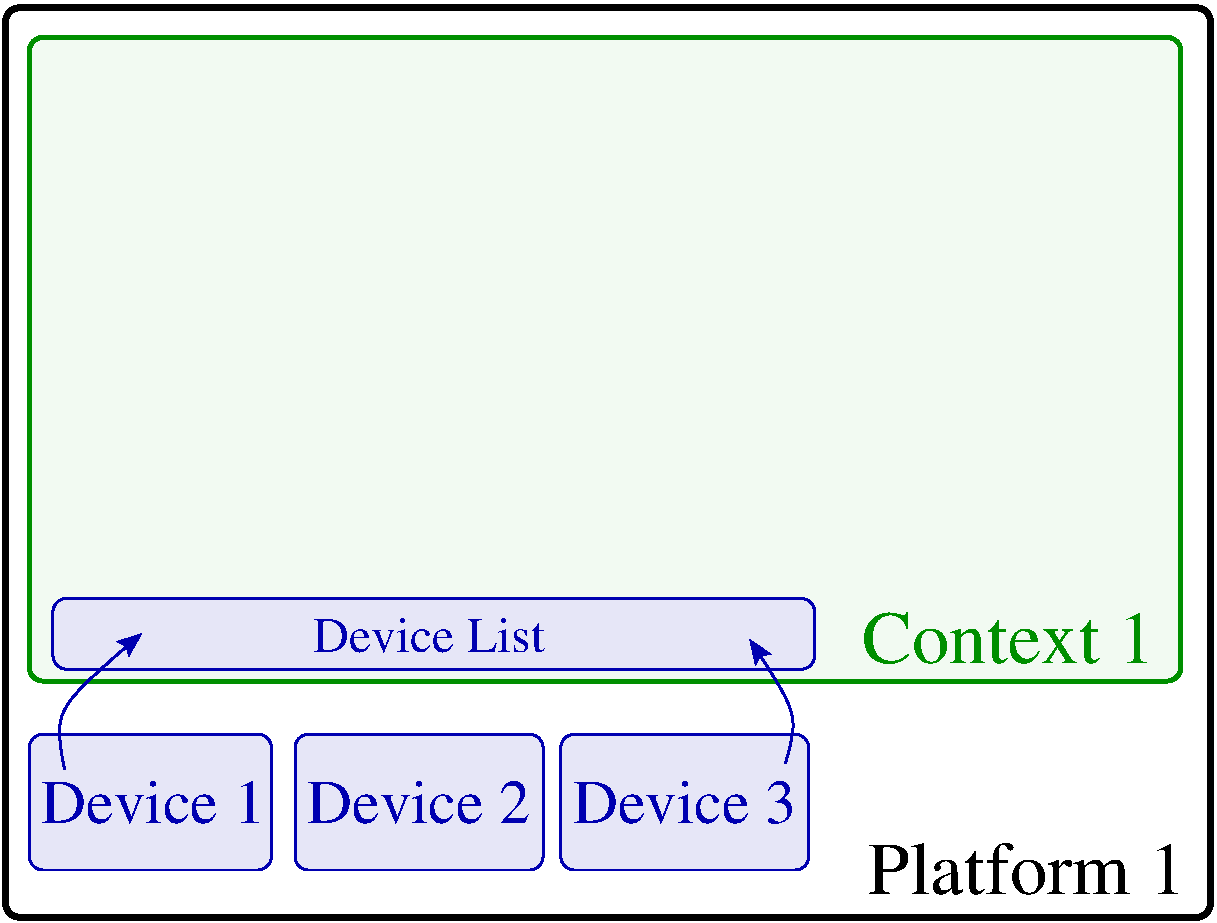
\includegraphics[width=0.80\textwidth]{figures/opencl-5.pdf}
%  \end{center}
% \end{frame}
% 
% \begin{frame}{OpenCL Platform Model}
%  \begin{center}
%    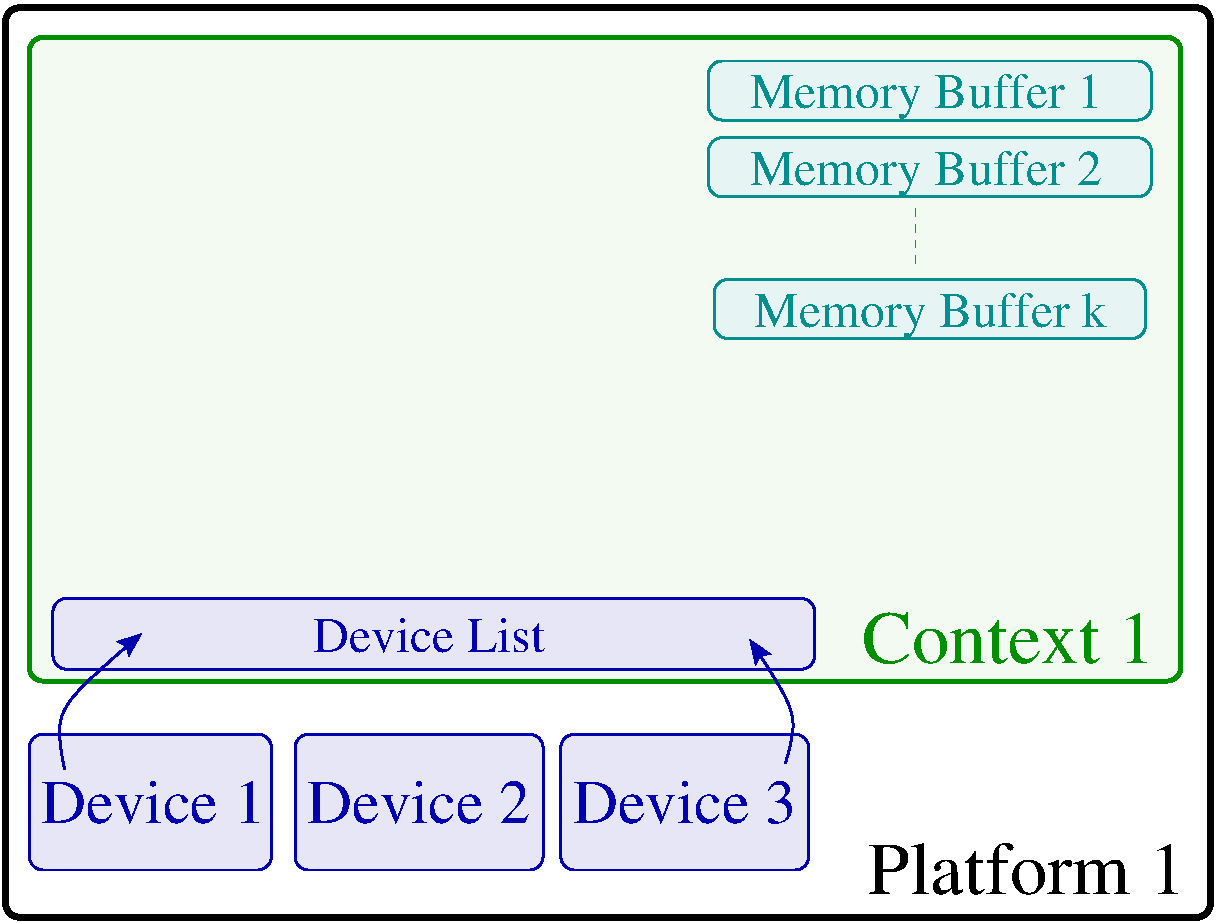
\includegraphics[width=0.80\textwidth]{figures/opencl-6.pdf}
%  \end{center}
% \end{frame}
% 
% \begin{frame}{OpenCL Platform Model}
%  \begin{center}
%    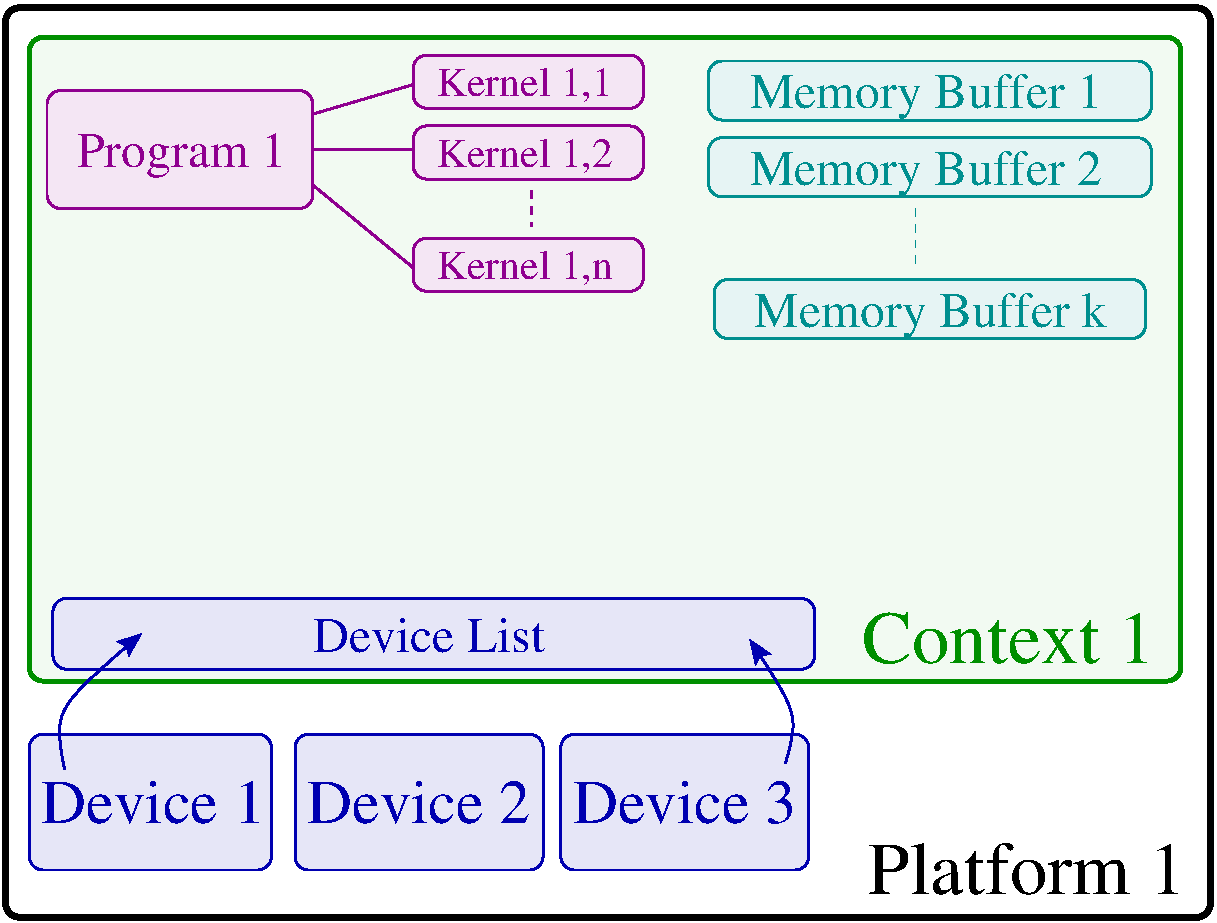
\includegraphics[width=0.80\textwidth]{figures/opencl-7.pdf}
%  \end{center}
% \end{frame}
% 
% \begin{frame}{OpenCL Platform Model}
%  \begin{center}
%    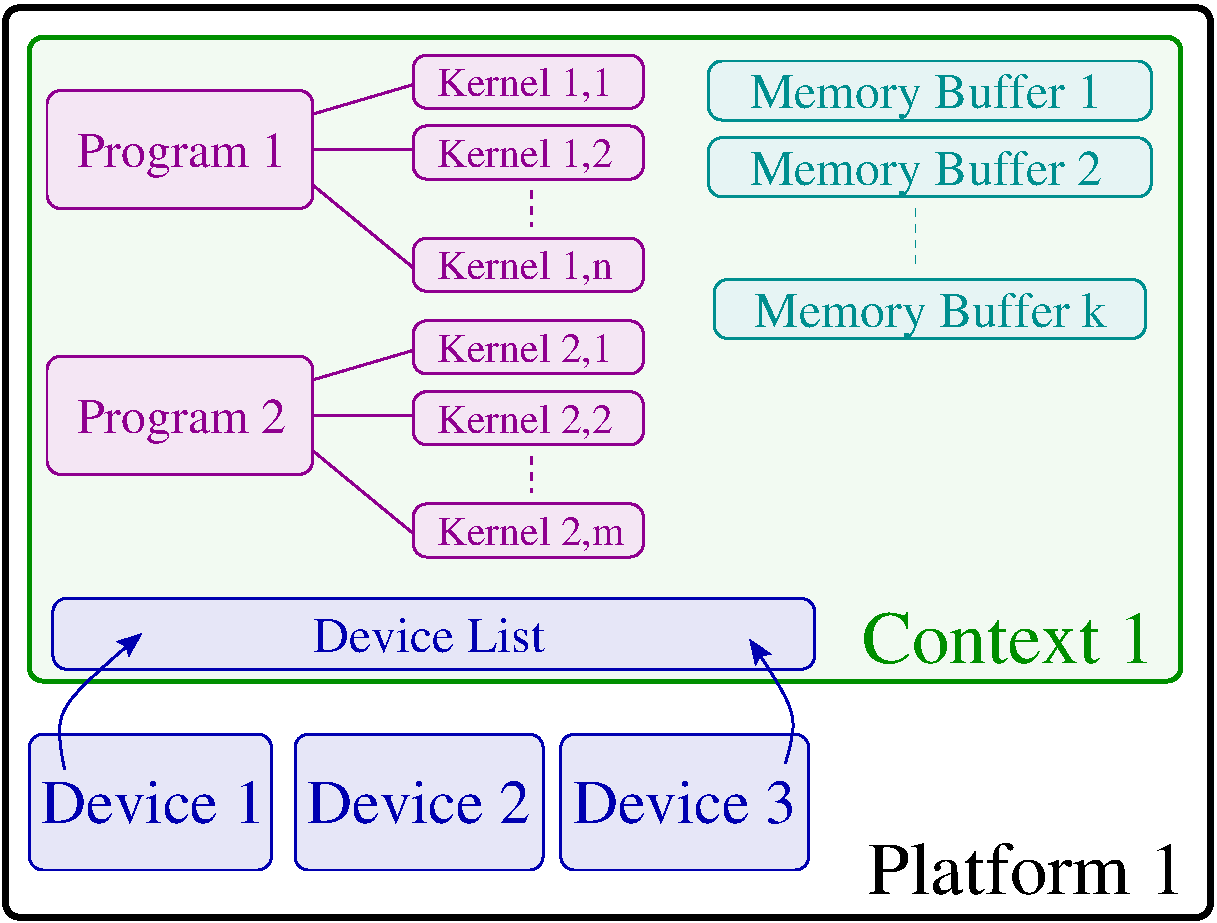
\includegraphics[width=0.80\textwidth]{figures/opencl-8.pdf}
%  \end{center}
% \end{frame}

\begin{frame}{OpenCL Platform Model}
 \begin{center}
   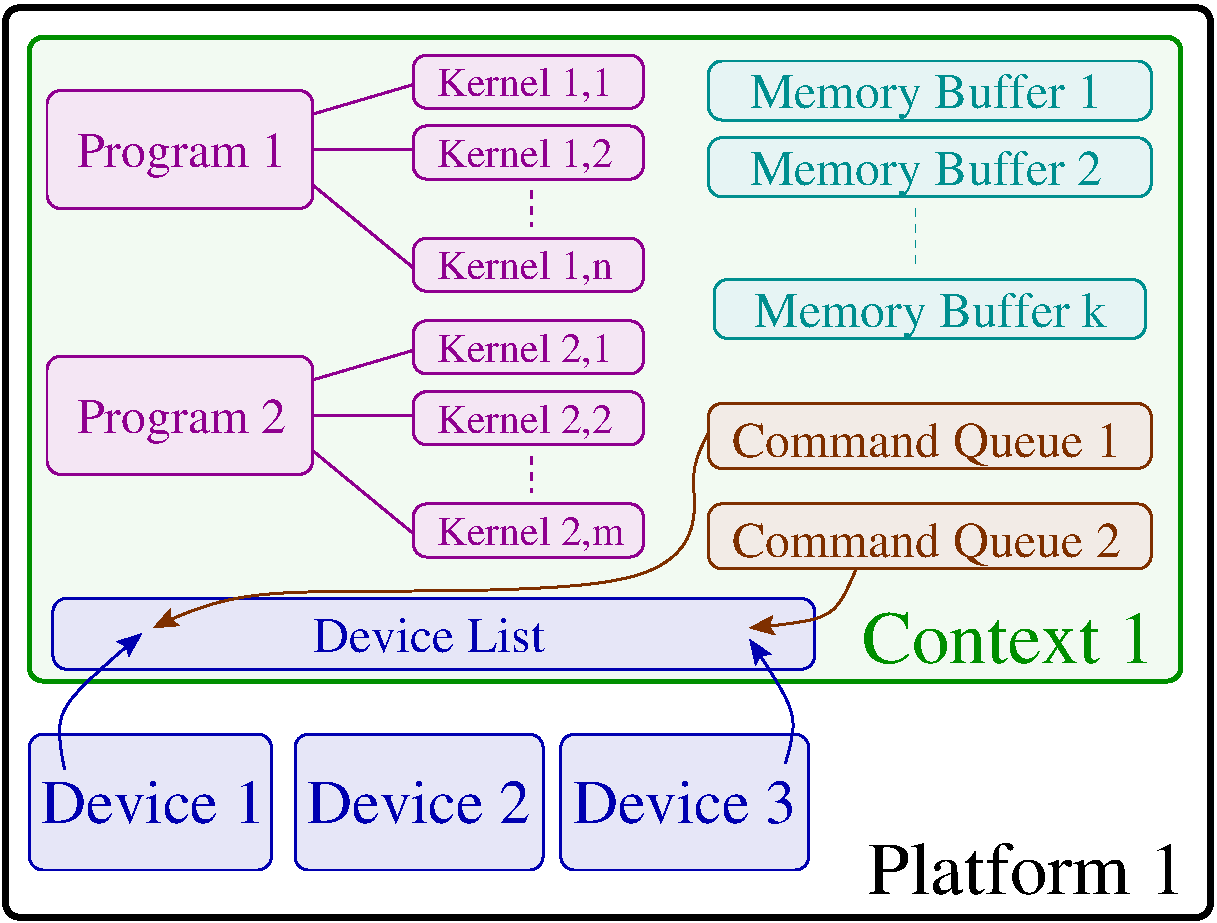
\includegraphics[width=0.80\textwidth]{figures/opencl-full.pdf}
 \end{center}
\end{frame}


% Explain differences to CUDA

\begin{frame}{OpenCL}

\begin{minipage}{0.7\textwidth}
\begin{block}{OpenCL Thread Control (1D) vs. CUDA}
 \begin{itemize}
  \item Local ID in block: \lstinline|get_local_id(0)|
  \item Threads per block: \lstinline|get_local_size(0)|
  \item ID of block: \lstinline|get_group_id()|
  \item No. of blocks: \lstinline|get_num_groups()|
  \item Global thread ID: \lstinline|get_global_id()|
  \item No. of threads: \lstinline|get_global_size()|
 \end{itemize}
\end{block}
\end{minipage}
\begin{minipage}{0.25\textwidth}
\begin{block}{}
 \begin{itemize}
  \item {\color{darkgreen}\lstinline|threadIdx.x|}
  \item {\color{darkgreen}\lstinline|blockDim.x|}
  \item {\color{darkgreen}\lstinline|blockIdx.x|}
  \item {\color{darkgreen}\lstinline|gridDim.x|}
  \item
 \end{itemize}
\end{block}
\vspace*{0.1cm}
\end{minipage}

\end{frame}




%%% Conclusion



\begin{frame}{Conclusion}

 \begin{block}{Just-In-Time Kernel Compilation}
   \begin{itemize}
    \item Require optional kernel caching by OpenCL SDKs
   \end{itemize}
 \end{block}

 \begin{block}{Kernel Interaction}
   \begin{itemize}
    \item Allow calling host functions for OpenCL kernels on CPU
   \end{itemize}
 \end{block}

  \begin{block}{OpenCL Heterogeneity}
   \begin{itemize}
    \item Let OpenCL benefit from Vulkan's momentum
   \end{itemize}
 \end{block}
\end{frame}
